\section {Results}
\label{sec:results}

In this work, we experimented on 3 software programs (SvmLight binary classifier, ScikitLearn binary classifier 
(which provides probabilities for each data point after classification) and ScikitLearn predictor 
(which classifies data point, aggregates the results and provides a final predicted label for each element)) 
for performing classification through the settings described in the section~\ref{sec:materials}. 
We experimented on datasets with 7 and 8 classes of sequences through shuffled, balanced and downsampled settings. 
The study also includes results from Micro and Macro averaging techniques through 3 different aggregation methodology 
for final label prediction.

Table \ref{tab:table1} shows the average accuracy, sensitivity, specificity and Mathews correlation coefficient values 
for amino acid composition (AAC) for models with 7 and 8 classes in their dataset when results are classified and predicted 
using ScikitLearn predictor program. Table \ref{tab:table4} and Table \ref{tab:table5} on the other hand, 
shows the average accuracy, sensitivity, specificity and Mathews correlation coefficient values for amino acid composition (AAC) 
for models with 7 (Table 2) and 8 (Table 3) classes in their dataset when results are classified using SvmLight 
and ScikitLearn binary classifiers programs.

Overall, models with 8 classes of protein sequences in the dataset perform better and provide higher numerical values 
compared to the ones with 7 classes of proteins in the dataset. The 8-class based datasets contain more sequences and 
thus there are more data available for the classification algorithm to learn from which leads to better performance results.

Regrading the different aggregation techniques, the vote-based models corresponds to multi-class classification 
problems where there is one predicted label for each element in the dataset. For the problems in this category, 
the results from all 3 software programs are very close through the same settings. We suggest the ScikitLearn predictor 
since it involves less coding and thus provides better reproducibility when merged with other tools from the ScikitLearn Library.

The class-based and threshold-based models correspond to the multi-label classification problems where there can 
be more than one predicted label for an element of the dataset. The difference is that, on class-based aggregation technique, 
the specificity-sensitivity value pairs, initially show a considerable difference(the difference amount depends on 
the software used for classification), wherein threshold-based technique we need to apply a threshold to 
the predicted results to put the specificity-sensitivity value pairs in balance.

Overall for both SvmLight and ScikitLearn binary classifiers, the closest results to the original ones are achieved through 
threshold-based aggregation technique on shuffled and balanced datasets when the metrics are Micro averaged.

ScikitLearn predictor program could not be used for class-based and threshold-based aggregation techniques because 
it aggregates and provides one label result for each element. If you want to use ScikitLearn support vector machine 
classier for these models (which is the case for problems like the work in~\cite{mishra2014prediction}) 
you need to use it as a binary classifier that provides the probability for each point and you can manage the 
aggregation technique on your own depending on the problem requirements (Table 2 and 3, ScikitLearn binary classifier).

Regarding the 2 different settings for Gamma and Cost values, compared to applying on single value pair to all classes 
of the dataset, applying different value pairs to each involved class, increases the chance of obtaining more true 
positives and thus better results. But through this work, we didn’t observe a considerable difference in between the 
results through any of those 2 settings mentioned above.

Regarding Micro versus Macro averaging techniques, Micro averaging provides higher MCC values and less difference in between 
sensitivity and specificity for almost all the models but it does not affect the accuracy greatly. Also, for balanced 
datasets (down-sampled instance), although using different averaging techniques affects the results but the impact 
is not as much as it is for imbalanced instances of the datasets (shuffled and balanced).

Regarding different instances of the dataset, the performance metric results of the balanced and shuffled 
instances of the dataset are close, where for down-sampled version of the dataset we observed lower 
values for performance metrics since compared to the balanced and shuffled instances, the down-sampled version 
contains less proteins sequences which mean less data for training the classifier.


Figure~\ref{fig:figure7} and Figur ~\ref{fig:figure8} are the specificity-sensitivity contour density plot of all 
the models built on datasets containing 7 (figure 1) and 8 (figure 2) classes of proteins. The results fit themselves 
into 3 different groups. 

The first group include the data points with the least distance to the initial results which are the results being 
achieved using threshold-based aggregation technique classified by either SvmLight or ScikitLearn binary classifiers. 
The Micro averaged results appear closer to the initial results where the Macro averaged ones appear farther but 
still in the same group. For 8 class based models (figure 8), closest results appear a bit farther from the initial 
results because they provide better results (higher values) compared to the same models with 7 protein classes 
in the dataset.

The second group above the first one on the top, corresponds to the models with class-based aggregation technique when classified 
using ScikitLearn binary classifier. The observed difference in between specificity and sensitivity values in these models 
(compared to same models when classified using SvmLight program) is probably the product of the default threshold value 
of the classifier. This group in figure 8 still appear on the top left but not completely separated from the next group as their 
performance metric values does not differ greatly from the next group. 
The third group in between these two, corresponds to all the other models of the experiment.

Table \ref{tab:table6} shows the average accuracy, sensitivity, specificity and Mathews correlation coefficient values 
from our best model setting being applied to all the features being mentioned in the table 1 of the 
initial study~\cite{mishra2014prediction}.

% Figure 1
\begin{figure}
    \begin{small}
        \begin{center}
            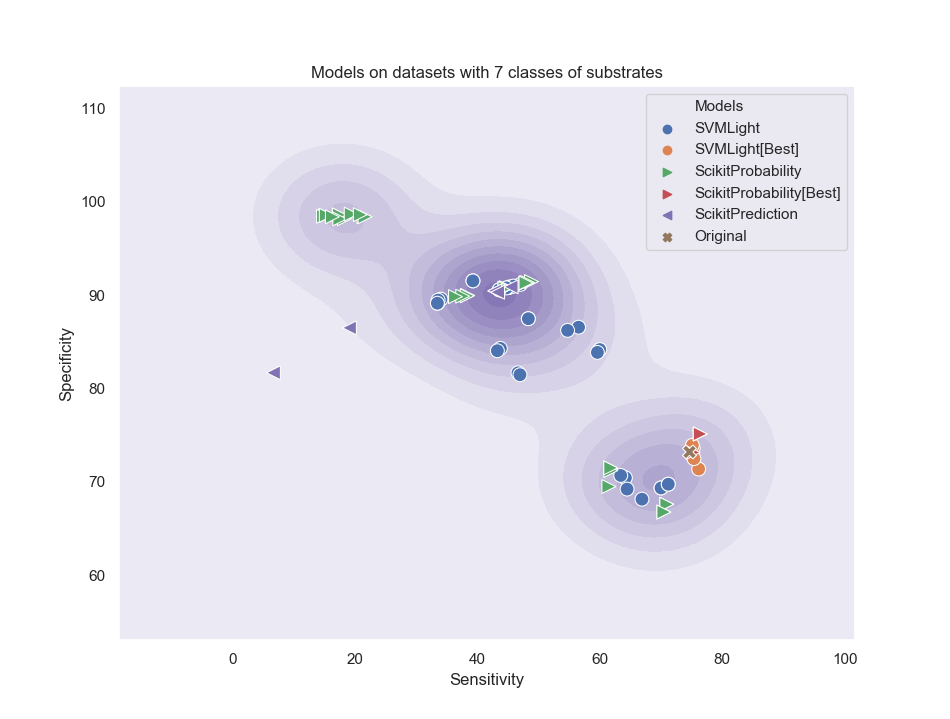
\includegraphics[width=0.8\textwidth]{figures/fig71}
        \end{center}
        \caption{Models with 7 classes of proteins in the dataset}
        \label{fig:figure7}
    \end{small}
\end{figure}

% Figure 2
\begin{figure}
    \begin{small}
        \begin{center}
            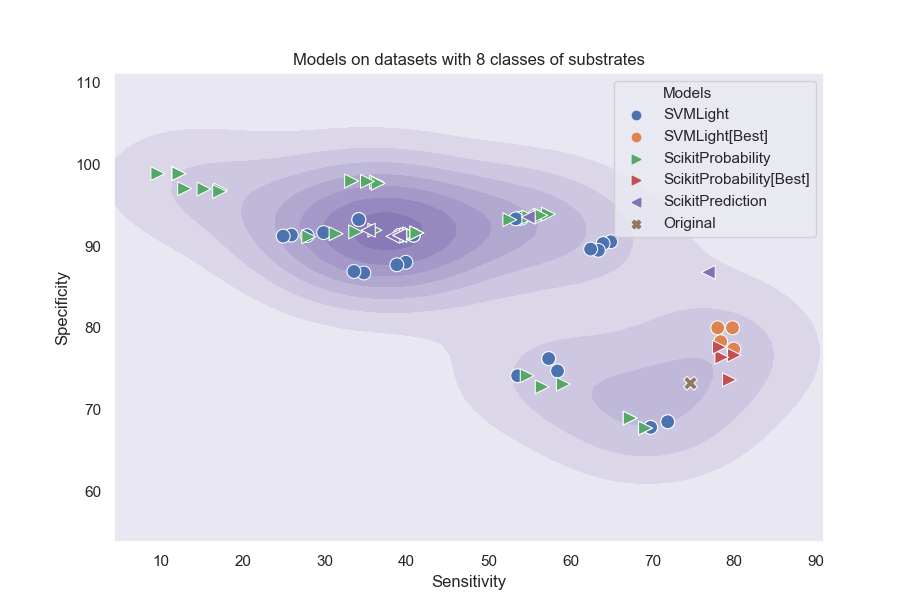
\includegraphics[width=0.8\textwidth]{figures/fig81}
        \end{center}
        \caption{Models with 8 classes of proteins in the dataset}
        \label{fig:figure}
    \end{small}
\end{figure}

% Table 1

\begin{table}[ht]
    \centering
    \begin{tabular}{|L | V |V V V V g g g V V V V | V |}
        \hline
        \multicolumn{14}{|g|}{Scikit-learn prediction-based models}\\
        \hline
        \multicolumn{1}{|l|}{\multirow{2}{*}{\footnotesize{Original Results}}}
        &
        \multicolumn{3}{g}{Accuracy} & \multicolumn{3}{g}{Sensitivity} &
        \multicolumn{3}{g}{Specificity} & \multicolumn{4}{g|}{MCC}\\
        \cline{2-14}&
        \multicolumn{3}{C}{73.74} & \multicolumn{3}{C}{74.65} &
        \multicolumn{3}{C}{73.22} & \multicolumn{4}{C|}{0.46} \\
        \hline
        
        \cline{1-12}\multicolumn{1}{|g}{}&
        
        \multicolumn{1}{|g|}{\footnotesize{Dist}}&
        \multicolumn{4}{g} {\footnotesize{7 class-based models}}&
        \multicolumn{3}{g}{}&
        \multicolumn{4}{g|} {\footnotesize{8 class-based models}}&
        \multicolumn{1}{g|}{\footnotesize{Dist}}\\
        
        \cline{3-6}\cline{10-13}\multicolumn{1}{|g}{}&
        \multicolumn{1}{|g|}{\footnotesize{ance}}&
        \multicolumn{1}{g}{acc}&\multicolumn{1}{g}{sens}&
        \multicolumn{1}{g}{spec}&\multicolumn{1}{g}{mcc}&
        \multicolumn{3}{g}{}&
        \multicolumn{1}{g}{acc}&\multicolumn{1}{g}{sens}&
        \multicolumn{1}{g}{spec}&\multicolumn{1}{g|}{mcc}&\multicolumn{1}{g|}{\footnotesize{ance}}\\

        \hline

        \multicolumn{1}{|l|}{\multirow{6}{*}{\footnotesize{Prediction-based}}}
        
        & 0.70 & 76.88 & 19.10 & 86.51 & 0.05 &    s&&s                & 84.58 & 38.33 & 91.19 & 0.29 & 0.45 \\
        & 0.39 & 83.66 & 42.86 & 90.47 & 0.33 &    d&\small{Micro}&d   & 84.79 & 39.16 & 91.31 & 0.30 & 0.44 \\
        & \mrkm{0.36}{84.43}{45.51}{90.91}{0.36}&    sh&&sh              & \mrkm{88.71}{54.85}{93.54}{0.48}{0.32} \\

        
        \cline{2-5}\cline{7-9}\cline{11-14}
        
        & 0.81 & 76.88 & 6.69 & 81.70 & 0.01 &    s&&s                & 84.58 & 76.82 & 86.79 & 0.03 & 0.81 \\
        & 0.39 & 83.67 & 42.85 & 90.47 & 0.32 &    d&\small{Macro}&d   & 84.79 & 39.16 & 91.31 & 0.29 & 0.44 \\
        & 0.39 & 85.27 & 43.31 & 90.33 & 0.35 &    sh&&sh              & 88.71 & 35.32 & 91.94 & 0.29 & 0.48 \\
        
        \hline\hline
        
        \multicolumn{14}{|c|} {\footnotesize{
            S, D and SH are sorted, down-sampled and shuffled instances of the main dataset.
        }}\\
        \multicolumn{14}{|c|} {\footnotesize{
            Acc: Accuracy, Sens: Sensitivity, Spec: Specificity, Mcc: Matthews correlation coefficient
        }}\\

        \hline
        
       

    \end{tabular}
    \captionsetup{font=small,width=14cm}
    \caption{The average sensitivity, specificity, accuracy, and MCC values 
    for scikit-learn prediction-based models for amino acid composition (AAC).}
    \label{tab:table1}
    
\end{table}

\begin{table}[ht]
    \centering
    \begin{tabular}{|L |V V V V g g g V V V V |}
        \hline
        \multicolumn{12}{|g|}{7-class based model for AAC}\\
        \hline
        \multicolumn{1}{|l|}{\multirow{2}{*}{\footnotesize{Original Results}}}
        &
        \multicolumn{2}{g}{Accuracy} & \multicolumn{3}{g}{Sensitivity} &
        \multicolumn{3}{g}{Specificity} & \multicolumn{3}{g|}{MCC}\\
        \cline{2-12}&
        \multicolumn{2}{C}{73.74} & \multicolumn{3}{C}{74.65} &
        \multicolumn{3}{C}{73.22} & \multicolumn{3}{C|}{0.46} \\
        \hline\hline
        
        \multicolumn{12}{|g|} {SVM Light}\\
        \hline\hline
        \cline{1-12}\multicolumn{1}{|g}{}&
        \multicolumn{4}{g} {Gamma-Cost different for each class}&
        \multicolumn{3}{g}{}&
        \multicolumn{4}{g|} {same Gamma-Cost for all classes}\\
        \cline{2-5}\cline{9-12}\multicolumn{1}{|g}{}&
        \multicolumn{1}{g}{accuracy}&\multicolumn{1}{g}{sensitivity}&
        \multicolumn{1}{g}{specificity}&\multicolumn{1}{g}{mcc}&
        \multicolumn{3}{g}{}&
        \multicolumn{1}{g}{accuracy}&\multicolumn{1}{g}{sensitivity}&
        \multicolumn{1}{g}{specificity}&\multicolumn{1}{g|}{mcc}\\
        \hline

        \multicolumn{1}{|l|}{\multirow{6}{*}{\footnotesize{Before Voting}}}
        
        & 82.28 & 56.53 & 86.58 & 0.37 &    n&&n                & 80.73 & 60.00 & 84.18 & 0.37 \\
        & 84.07 & 39.28 & 91.55 & 0.32 &    d&\small{Micro}&d   & 81.90 & 48.33 & 87.5 & 0.32 \\
        & 81.74 & 54.74 & 86.24 & 0.36 &    sh&&sh              & 80.42 & 59.61 & 83.88 & 0.36 \\
        
        \cline{3-4}\cline{6-8}\cline{10-11}
        
        & 82.28 & 43.76 & 84.31 & 0.31 &    n&&n                & 80.73 & 46.64 & 81.69 & 0.30 \\
        & 84.08 & 39.28 & 91.54 & 0.32 &    d&\small{Macro}&d   & 81.90 & 48.33 & 87.49 & 0.33 \\
        & 81.73 & 43.27 & 84.06 & 0.28 &    sh&&sh              & 80.42 & 46.96 & 81.49 & 0.29 \\
        
        \hline
        \multicolumn{1}{|l|}{\multirow{6}{*}{\footnotesize{Thresholding}}}

        & 74.04 & 74.74 & 73.93 & 0.36 &    n&&n                & 73.07 & 76.66 & 72.47 & 0.36 \\
        & 72.89 & 66.66 & 73.92 & 0.30 &    d&\small{Micro}&d   & 69.96 & 71.19 & 69.76 & 0.29 \\
        & 73.88 & 72.18 & 74.16 & 0.34 &    sh&&sh              & 72.91 & 75.38 & 72.50 & 0.35 \\
        
        \cline{3-4}\cline{6-8}\cline{10-11}

        & 74.04 & 63.58 & 70.80 & 0.28 &    n&&n                & 73.07 & 65.34 & 69.17 & 0.27 \\
        & 72.89 & 66.66 & 73.92 & 0.30 &    d&\small{Macro}&d   & 69.96 & 71.19 & 69.76 & 0.30 \\
        & 73.88 & 62.26 & 71.01 & 0.27 &    sh&&sh              & 72.91 & 64.46 & 69.24 & 0.26 \\
        
        \hline
        \multicolumn{1}{|l|}{\multirow{6}{*}{\footnotesize{After Voting}}}

        & 84.87 & 47.05 & 91.17 & 0.38 &    n&&n                & 84.54 & 45.89 & 90.98 & 0.36 \\
        & 84.35 & 45.24 & 90.87 & 0.36 &    d&\small{Micro}&d   & 83.87 & 43.57 & 90.59 & 0.34 \\
        & 84.32 & 45.12 & 90.85 & 0.35 &    sh&&sh              & 84.21 & 44.74 & 90.79 & 0.35 \\
        
        \cline{3-4}\cline{6-8}\cline{10-11}

        & 84.87 & 34.05 & 89.58 & 0.28 &    n&&n                & 84.54 & 33.59 & 89.48 & 0.27 \\
        & 84.35 & 45.23 & 90.87 & 0.34 &    d&\small{Macro}&d   & 83.87 & 43.57 & 90.59 & 0.33 \\
        & 84.32 & 33.52 & 89.14 & 0.27 &    sh&&sh              & 84.21 & 33.47 & 89.15 & 0.27 \\
        
        \hline\hline
        
        \multicolumn{12}{|g|} {Scikit Learn}\\
        \hline\hline

        \multicolumn{1}{|l|}{\multirow{6}{*}{\footnotesize{Before Voting}}}
        
        & 87.42 & 34.10 & 96.30 & 0.39 &    n&&n                & 80.25 & 30.90 & 88.48 & 0.19 \\
        & 87.07 & 24.28 & 97.53 & 0.33 &    d&\small{Micro}&d   & 86.62 & 25.00 & 96.90 & 0.31\\
        & 86.75 & 31.92 & 95.90 & 0.36 &    sh&&sh              & 87.01 & 30.89 & 96.36 & 0.36\\
        
        \cline{3-4}\cline{6-8}\cline{10-11}
        
        & 87.41 & 28.70 & 95.77 & 0.34 &    n&&n                 & 87.20 & 24.18 & 96.06 & 0.28 \\
        & 87.07 & 24.28 & 97.53 & 0.30 &    d&\small{Macro}&d   & 86.63 & 25.00 & 96.90 & 0.28 \\
        & 86.75 & 26.20 & 95.36 & 0.29 &    sh&&sh              & 87.014 & 24.19 & 95.84 & 0.27 \\
        
        \hline
        \multicolumn{1}{|l|}{\multirow{6}{*}{\footnotesize{Thresholding}}}

        & 74.52 & 35.26 & 81.07 & 0.14 &    n&&n                & 75.07 & 31.54 & 82.33 & 0.12 \\
        & 80.13 & 24.52 & 89.40 & 0.14 &    d&\small{Micro}&d   & 79.25 & 25.00 & 88.29 & 0.13\\
        & 73.07 & 32.81 & 79.78 & 0.10 &    sh&&sh               & 73.90 & 31.66 & 80.94 & 0.11\\
        
        \cline{3-4}\cline{6-8}\cline{10-11}

        & 74.52 & 30.74 & 81.54 & 0.13 &    n&&n                & 75.07 & 25.34 & 82.74 & 0.09\\
        & 80.13 & 24.52 & 89.40 & 0.17 &    d&\small{Macro}&d   & 79.24 & 25.00 & 88.29 & 0.15\\
        & 73.07 & 27.74 & 80.28 & 0.09 &    sh&&sh              & 73.90 & 25.36 & 81.40 & 0.08 \\
        
        \hline
        \multicolumn{1}{|l|}{\multirow{6}{*}{\footnotesize{After Voting}}}

        & 81.28 & 34.49 & 89.08 & 0.24 &    n&&n                & 80.25 & 30.90 & 88.49 & 0.19\\
        & 78.84 & 25.95 & 87.65 & 0.13 &    d&\small{Micro}&d   & 79.18 & 27.14 & 87.86 & 0.15\\
        & 80.66 & 32.308 & 88.72 & 0.21&    sh&&sh              & 80.51 & 31.79 & 88.63 & 0.20\\
        
        \cline{3-4}\cline{6-8}\cline{10-11}

        & 81.28 & 29.66 & 89.07 & 0.19 &    n&&n                & 80.26 & 24.75 & 88.53 & 0.13 \\
        & 78.84 & 25.95 & 87.65 & 0.14&     d&\small{Macro}&d   & 79.18 & 27.14 & 87.85 & 0.14\\
        & 80.65 & 27.29 & 88.71 & 0.15 &    sh&&sh              & 80.51 & 25.97 & 88.65 & 0.14 \\
        \hline
        
       

    \end{tabular}
    \captionsetup{font=small,width=12cm}
    \caption{The average sensitivity, specificity, accuracy, and MCC from all the 
    models being built on 7 class-based dataset. n, d and sh are normal, 
    downsampled and shuffled instances of the main dataset.}
    \label{tab:table4}
    
\end{table}
\begin{table}[ht]
    \centering
    \begin{tabular}{|L | V |V V V V g g g V V V V | V |}
        \hline
        \multicolumn{14}{|g|}{8-class based model for AAC}\\
        \hline
        \multicolumn{1}{|l|}{\multirow{2}{*}{\footnotesize{Original Results}}}
        &
        \multicolumn{3}{g}{Accuracy} & \multicolumn{3}{g}{Sensitivity} &
        \multicolumn{3}{g}{Specificity} & \multicolumn{4}{g|}{MCC}\\
        \cline{2-14}&
        \multicolumn{3}{C}{73.74} & \multicolumn{3}{C}{74.65} &
        \multicolumn{3}{C}{73.22} & \multicolumn{4}{C|}{0.46} \\
        \hline\hline
        
        \multicolumn{14}{|g|} {SVM Light}\\
        \hline\hline
        
        \cline{1-12}\multicolumn{1}{|g}{}&
        
        \multicolumn{1}{|g|}{\footnotesize{Dist}}&
        \multicolumn{4}{g} {Gamma-Cost different for each class}&
        \multicolumn{3}{g}{}&
        \multicolumn{4}{g|} {same Gamma-Cost for all classes}&
        \multicolumn{1}{g|}{\footnotesize{Dist}}\\
        
        \cline{3-6}\cline{10-13}\multicolumn{1}{|g}{}&
        \multicolumn{1}{|g|}{\footnotesize{ance}}&
        \multicolumn{1}{g}{acc}&\multicolumn{1}{g}{sens}&
        \multicolumn{1}{g}{spec}&\multicolumn{1}{g}{mcc}&
        \multicolumn{3}{g}{}&
        \multicolumn{1}{g}{acc}&\multicolumn{1}{g}{sens}&
        \multicolumn{1}{g}{spec}&\multicolumn{1}{g|}{mcc}&\multicolumn{1}{g|}{\footnotesize{ance}}\\

        \hline

        \multicolumn{1}{|l|}{\multirow{6}{*}{\footnotesize{Class-based}}}
        
        & 0.24 & 87.33 & 64.92 & 90.53 & \mrko{0.49} &    b&&b               & 86.22 & 63.40 & 89.48 & 0.46 & 0.23 \\
        & 0.49 & 85.86 & 34.16 & 93.24 & 0.30 &    d&\small{Micro}&d   & 85.02 & 40.83 & 91.34 & 0.32 & 0.42 \\
        & 0.24 & 87.02 & 63.98 & 90.31 & 0.48 &    s&&s                & 86.24 & 62.46 & 89.63 & 0.46 & 0.23 \\
        
        \cline{2-5}\cline{7-9}\cline{11-14}
        
        & 0.43 & 87.33 & 39.91 & 88.02 & 0.30 &    b&&b               & 86.22 & 34.78 & 86.71 & 0.25 & 0.48 \\
        & 0.49 & 85.85 & 34.16 & 93.24 & 0.28 &    d&\small{Macro}&d   & 85.02 & 40.83 & 91.34 & 0.30 & 0.42 \\
        & 0.44 & 87.02 & 38.81 & 87.71 & 0.28 &    s&&s                & 86.24 & 33.57 & 86.89 & 0.23 & 0.50 \\
        
        \hline
        \multicolumn{1}{|l|}{\multirow{6}{*}{\footnotesize{Threshold-based}}}

        & \mrkm{0.10}{79.98}{79.78}{80.01}{0.44} &    b&&b               & \mrkm{79.74}{77.97}{80.00}{0.43}{0.10} \\
        & 0.19 & 68.93 & 71.87 & 68.51 & 0.27 &     d&\small{Micro}&d   & 68.07 & 69.79 & 67.82 & 0.25 & 0.22 \\
        & \mrkm{0.09}{77.71}{79.93}{77.40}{0.41} &     s&&s                & \mrkm{78.31}{78.33}{78.31}{0.41}{0.09} \\
        
        \cline{2-5}\cline{7-9}\cline{11-14}

        & 0.21 & 79.59 & 57.34 & 76.24 & 0.28 &    b&&b               & 79.59 & 57.34 & 76.24 & 0.28 & 0.25 \\
        & 0.19 & 68.93 & 71.87 & 68.51 & 0.27 &     d&\small{Macro}&d   & 68.07 & 69.79 & 67.82 & 0.25 & 0.22 \\
        & 0.21 & 77.71 & 53.55 & 74.14 & 0.27 &     s&&s                & 78.31 & 58.42 & 74.72 & 0.26. & 0.26 \\
        
        \hline
        \multicolumn{1}{|l|}{\multirow{6}{*}{\footnotesize{Vote-based}}}

        & 0.31 & 88.91 & 55.65 & 93.66 & \mrko{0.49} &    b&&b               & 88.51 & 54.05 & 93.43 & 0.47 & 0.32 \\
        & 0.43 & 84.84 & 39.37 & 91.33 & 0.30 &    d&\small{Micro}&d   & 84.79 & 39.16 & 91.30 & 0.30 & 0.44 \\
        & 0.32 & 88.44 & 53.76 & 93.39 & 0.47 &    s&&s                & 88.33 & 53.33 & 93.33 & 0.46 & 0.32 \\
        
        \cline{2-5}\cline{7-9}\cline{11-14}

        & 0.54 & 88.91 & 29.87 & 91.65 & 0.26 &    b&&b               & 88.51 & 25.93 & 91.35 & 0.22 & 0.58 \\
        & 0.44 & 84.84 & 39.37 & 91.34 & 0.29 &    d&\small{Macro}&d   & 84.79 & 39.16 & 91.31 & 0.28 & 0.44 \\
        & 0.57 & 88.44 & 27.85 & 91.28 & 0.23 &    s&&s                & 88.33 & 24.93 & 91.22 & 0.20 & 0.60 \\
        
        \hline
        \hline
        
        \multicolumn{14}{|g|} {Scikit Learn}\\
        \hline
        \hline

        \multicolumn{1}{|l|}{\multirow{6}{*}{\footnotesize{Class-based}}}
        
        & 0.48 & 90.22 & 36.33 & 97.84 & 0.46  &    b&&b               & 90.11 & 35.22 & 97.92 & 0.45 & 0.49 \\
        & 0.72 & 88.10 & 12.18 & 98.86 & 0.23 &    d&\small{Micro}&d   & 87.75 & 9.63 & 98.86 & 0.19 & 0.76  \\
        & 0.48 & 90.10 & 36.52 & 97.68 & 0.45 &    s&&s                & 89.89 & 33.28 & 97.96 & 0.43 & 0.50 \\
        
        \cline{2-5}\cline{7-9}\cline{11-14}
        
        & 0.68 & 90.19 & 17.30 & 96.85 & 0.22 &    b&&b               & 90.10 & 15.26 & 96.98 & 0.17 & 0.71 \\
        & 0.74 & 88.10 & 12.21 & 98.86 & 0.18 &    d&\small{Macro}&d   & 87.75 & 9.71 & 8.86 & 0.13 & 0.78  \\
        & 0.68 & 90.07 & 17.17 & 96.68 & 0.20 &    s&&s                & 89.88 & 12.90 & 97.02 & 0.15 & 0.74 \\
        
        \hline
        \multicolumn{1}{|l|}{\multirow{6}{*}{\footnotesize{Threshold-based}}}

        & \mrkm{0.08}{77.08}{80.0}{76.66}{0.40}  &     b&&b               & \mrkm{77.70}{78.18}{77.63}{0.40}{0.08} \\
        & 0.22 & 67.91 & 69.16 & 67.73 & 0.25 &     d&\small{Micro}&d   & 68.75 & 67.28 & 68.96 & 0.25 & 0.23  \\
        & \mrkm{0.08}{76.66}{78.47}{76.40}{0.39} &     s&&s                & 74.36 & 79.41 & 73.64 & 0.37 & 0.09 \\
        
        \cline{2-5}\cline{7-9}\cline{11-14}

        & 0.24 & 77.08 & 59.13 & 73.10 & 0.27 &     b&&b               & 77.70 & 54.72 & 74.14 & 0.25 & 0.28 \\
        & 0.21 & 67.91 & 69.16 & 67.73 & 0.26 &     d&\small{Macro}&d   & 68.75 & 67.29 & 68.95 & 0.26 & 0.22  \\
        & 0.27 & 76.66 & 56.55 & 72.78 & 0.25 &     s&&s                & 74.36 & 56.27 & 0.07 & 0.22 & 0.30 \\
        
        \hline
        \multicolumn{1}{|l|}{\multirow{6}{*}{\footnotesize{Vote-based}}}

        & 0.31 & 89.33 & 57.31 & 93.90 & \mrko{0.51} &     b&&b               & 88.73 & 54.92 & 93.56 & 0.48 & 0.32 \\
        & 0.42 & 85.10 & 40.41 & 91.49 & 0.31 &     d&\small{Micro}&d   & 85.31 & 41.25 & 91.60 & 0.32 & 0.41  \\
        & 0.31 & 89.09 & 56.37 & 93.76 & 0.50 &     s&&s                & 88.15 & 52.60 & 93.22 & 0.45 & 0.33 \\
        
        \cline{2-5}\cline{7-9}\cline{11-14}

        & 0.47 & 89.32 & 36.12 & 91.94 & 0.34 &     b&&b               & 88.73 & 31.39 & 91.51 & 0.29 & 0.52 \\
        & 0.43 & 85.10 & 40.41 & 91.48 & 0.30 &     d&\small{Macro}&d   & 85.31 & 41.25 & 91.60 & 0.31 & 0.42  \\
        & 0.49 & 89.09 & 33.78 & 91.73 & 0.30 &     s&&s                & 88.15 & 28.05 & 91.14 & 0.23 & 0.56 \\
        \hline\hline
        
        \multicolumn{14}{|c|} {\footnotesize{
            B, D and S are balanced, down-sampled and shuffled instances of the main dataset.
        }}\\
        \multicolumn{14}{|c|} {\footnotesize{
            Acc: Accuracy, Sens: Sensitivity, Spec: Specificity, Mcc: Matthews correlation coefficient
        }}\\

        \hline
        
       

    \end{tabular}
    \captionsetup{font=small,width=14cm}
    \caption{The average sensitivity, specificity, accuracy, and MCC  for 8 class-based models.}
    \label{tab:table5}
    
\end{table}



\begin{table}[ht]
    \centering

    \begin{tabular}{|L || g g g g || C C C C|}
    \hline
    \multicolumn{1}{|l||}{\multirow{2}{*}{Method}}
    &
    \multicolumn{4}{g||}{Paper's Results}
    &
    \multicolumn{4}{c|}{Reproduced Results}
    \\ \cline{2-5} \cline{6-9}
    \multicolumn{1}{|c||}{}
    &
    Sensitivity  &  Specificity  &  Accuracy  &  MCC
    &
    Sensitivity  &  Specificity  &  Accuracy  &  MCC
    \\
    \hline \hline
    AAC & 74.65 & 73.22 & 73.74 & 0.46      &    79.98 & 79.78 & 80.01 & 0.44 \\
    DPC & 71.36 & 71.17 & 71.32 & 0.40 & -- & -- & -- & --  \\
    PHC & 70.63 & 70.42 & 70.60 & 0.38 & -- & -- & -- & --  \\
    AAI & 71.54 & 71.98 & 71.80 & 0.40 & -- & -- & -- & --  \\
    PSSM & 74.00 & 76.03 & 75.48 & 0.47 & -- & -- & -- & --  \\
    \hline
    AAC + AAI & 73.84 & 73.36 & 73.37 & 0.44 & -- & -- & -- & --  \\
    AAC + PHC & 73.56 & 73.39 & 73.40 & 0.44 & -- & -- & -- & --  \\
    AAC + DPC & 73.01 & 74.23 & 73.85 & 0.44 & -- & -- & -- & --  \\
    AAC + PSSM & 72.33 &  74.62 &  73.87 &  0.44 & -- & -- & -- & --  \\
    DPC + PHC & 72.15 &73.13 &72.90 &0.43 & -- & -- & -- & --  \\
    DPC + AAI &    70.28  & 72.09 &  71.67 &  0.40 & -- & -- & -- & --  \\
    DPC + PSSM &69.87 &72.06 &71.37 &0.40& -- & -- & -- & --  \\
    AAI + PHC & 69.32 &  71.50 &  70.79 &  0.38 & -- & -- & -- & --  \\
    AAI + PSSM & 76.19 &77.17 &76.69& 0.49 & -- & -- & -- & -- \\
    \hline
    AAC + DPC + AAI & 73.01 &  74.32  & 73.89&   0.44 & -- & -- & -- & --  \\
    AAC + DPC + PHC & 73.04& 75.36   &74.75  & 0.46& -- & -- & -- & --  \\
    AAC + DPC + PSSM & 73.43 &73.73 &73.64 &0.44& -- & -- & -- & --  \\
    AAC + AAI + PHC & 73.01  & 73.82 &73.51 &  0.44& -- & -- & -- & --  \\
    AAC + AAI + PSSM & 72.34 &  74.62& 73.90 &  0.44 & -- & -- & -- & --  \\
    \hline \hline
    \multicolumn{9}{|c|}{\multirow{3}{*}{\footnotesize AAC:amino acid composition, 
    DPC:dipeptide composition, PHC:physico-chemical class composition,}}\\
    \multicolumn{9}{|c|}{}\\
    \multicolumn{9}{|c|}{\footnotesize AAI:biochemical composition(AAIndex), PSSM:position specific scoring matrix}\\
    \hline
    \end{tabular}
    
    \captionsetup{font=small,width=12cm}
    \caption{The average sensitivity, specificity, accuracy, and MCC for all seven 
    substrate-specific transporter classes for different SVM models on main dataset 
    comparing original results with the results from our best reproduced model}
    \label{tab:table6}
\end{table}